\begin{figure}
\centering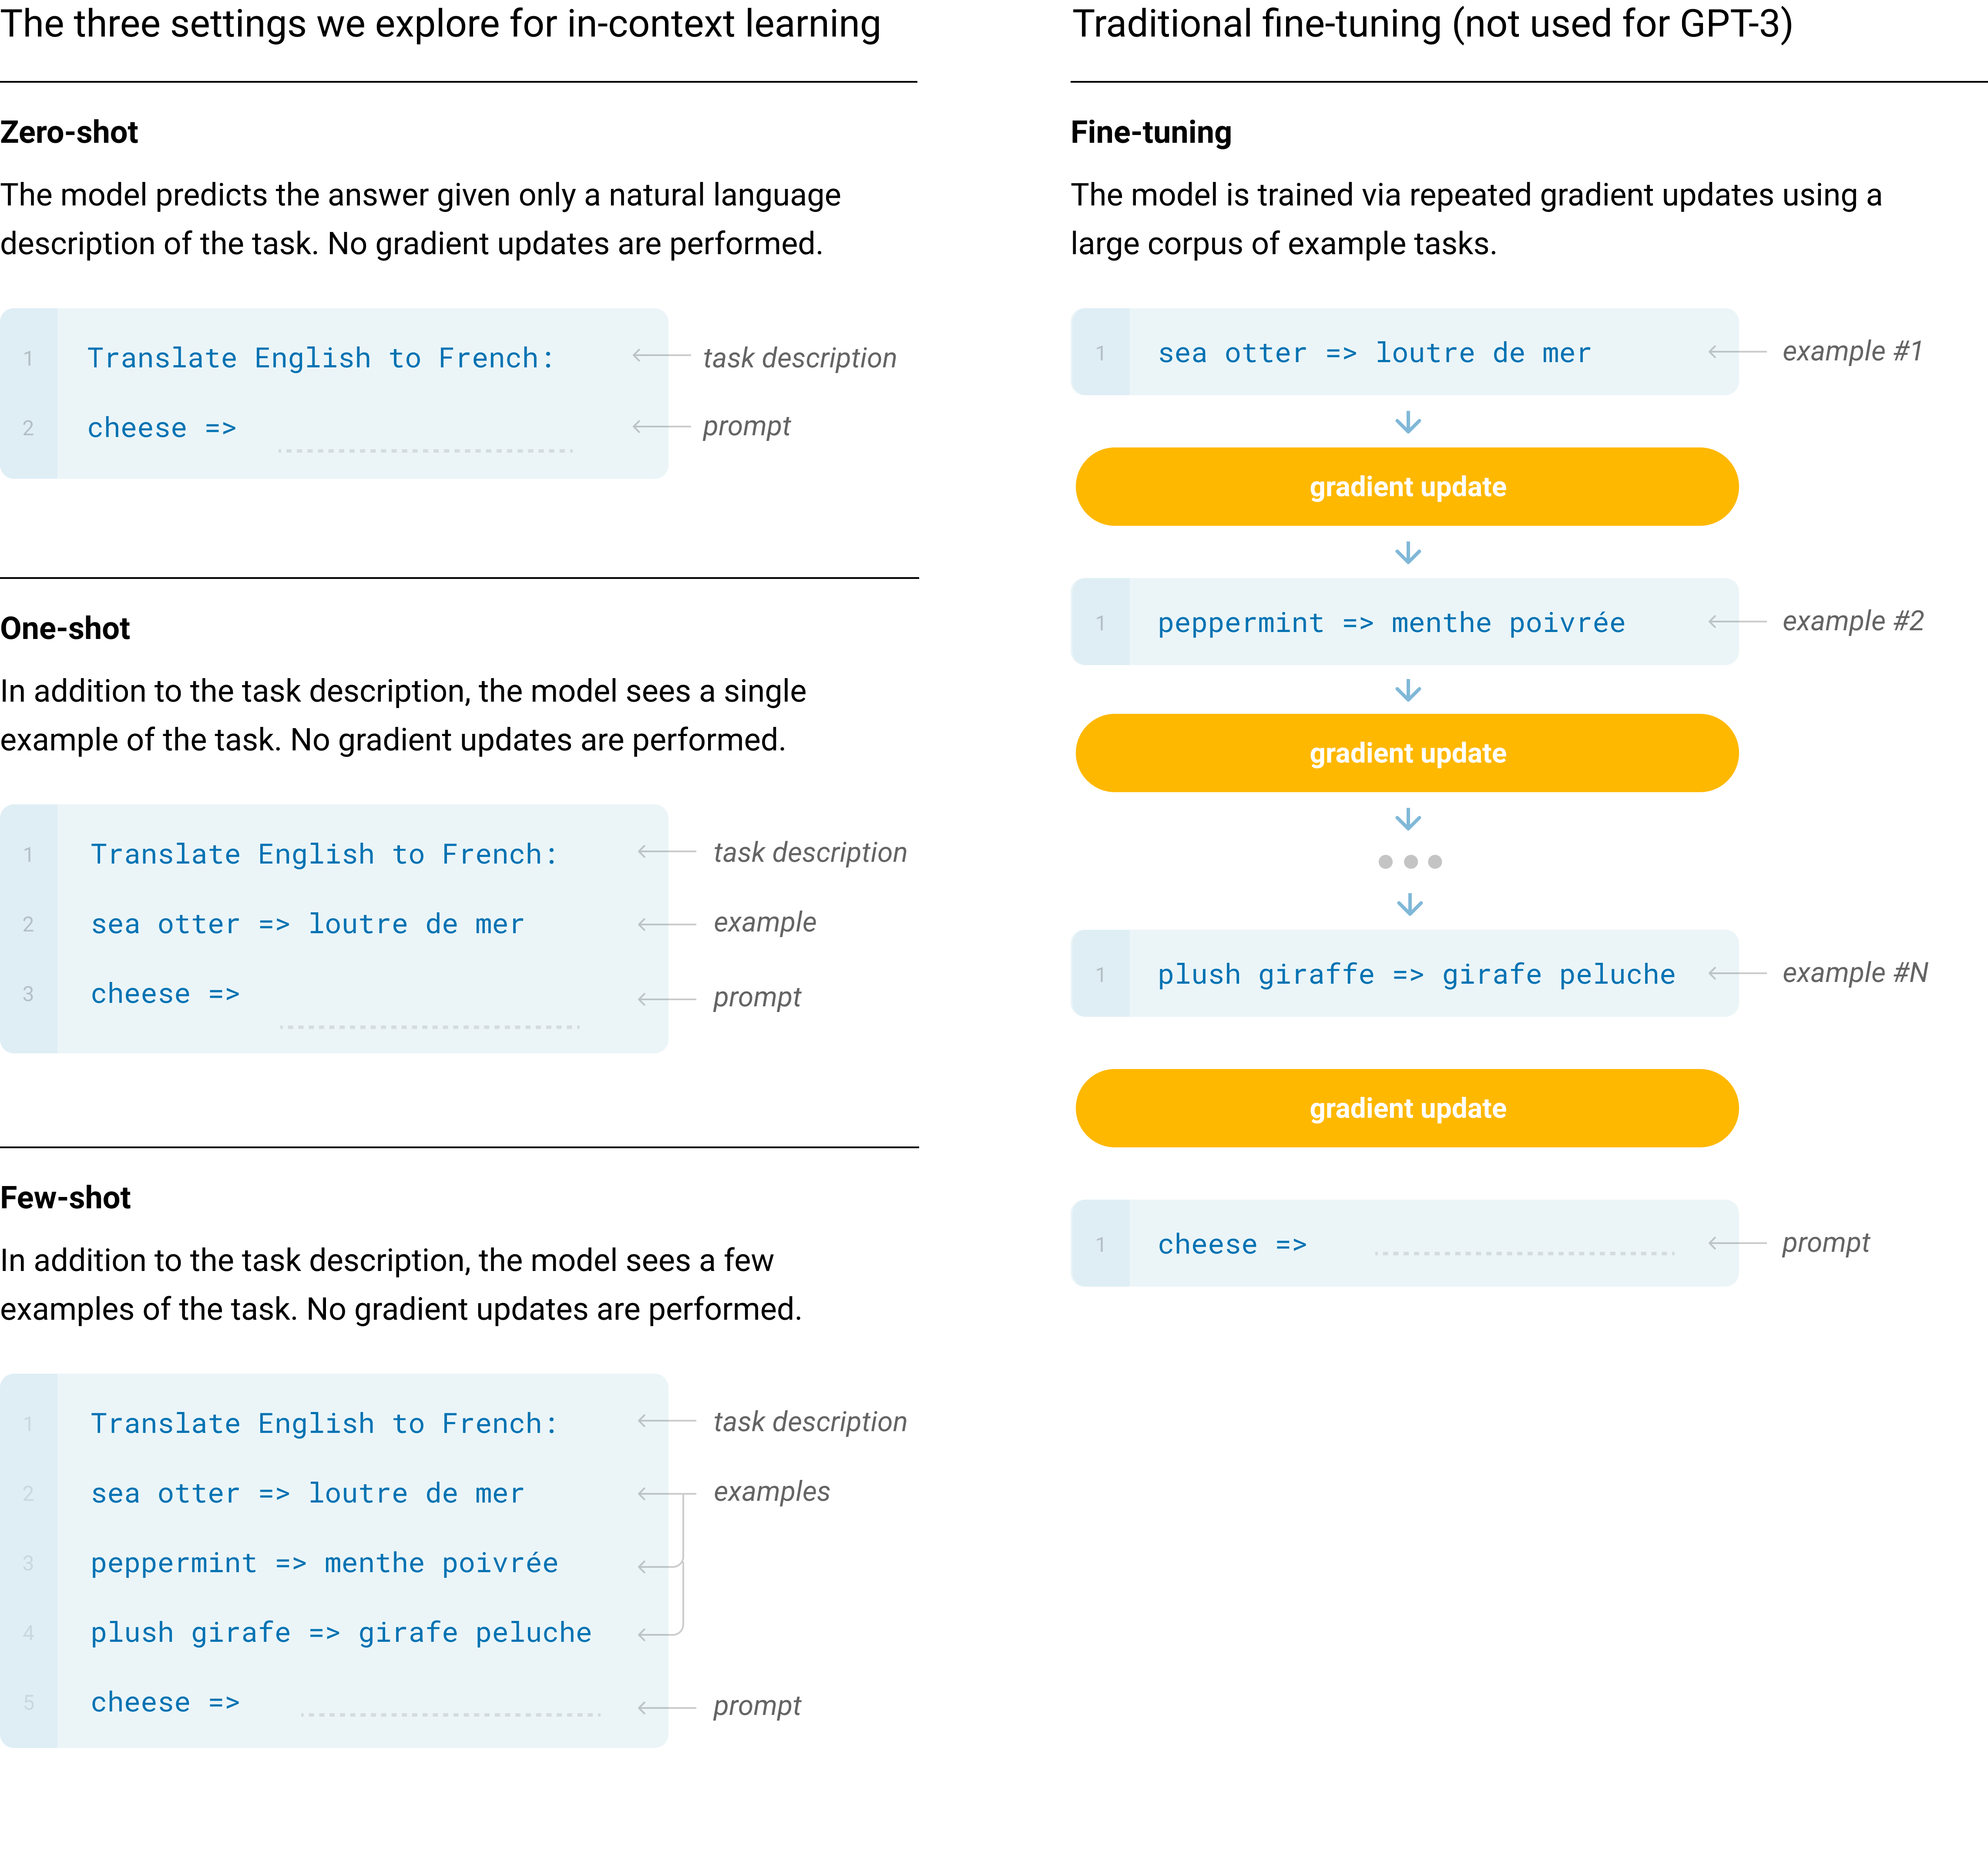
\includegraphics[width=0.8\linewidth]{figures/eval_strategies.png}
\caption{\textbf{Zero-shot, one-shot and few-shot, contrasted with traditional fine-tuning}. The panels above show four methods for performing a task with a language model -- fine-tuning is the traditional method, whereas zero-, one-, and few-shot, which we study in this work, require the model to perform the task with only forward passes at test time. We typically present the model with a few dozen examples in the few shot setting. Exact phrasings for all task descriptions, examples and prompts can be found in Appendix \ref{appendix:task_phrasing}.
}
\label{figure:eval strategies}
\end{figure}

Our basic pre-training approach, including model, data, and training, is similar to the process described in \cite{radford2019language}, with relatively straightforward scaling up of the model size, dataset size and diversity, and length of training.  Our use of in-context learning is also similar to \cite{radford2019language}, but in this work we systematically explore different settings for learning within the context.  Therefore, we start this section by explicitly defining and contrasting the different settings that we will be evaluating GPT-3 on or could in principle evaluate GPT-3 on. These settings can be seen as lying on a spectrum of how much task-specific data they tend to rely on.  Specifically, we can identify at least four points on this spectrum (see Figure \ref{figure:eval strategies} for an illustration):

\begin{itemize}
    \item \textbf{Fine-Tuning (FT)} has been the most common approach in recent years, and involves updating the weights of a pre-trained model by training on a supervised dataset specific to the desired task.  Typically thousands to hundreds of thousands of labeled examples are used.  The main advantage of fine-tuning is strong performance on many benchmarks. The main disadvantages are the need for a new large dataset for every task, the potential for poor generalization out-of-distribution \cite{mccoy2019right}, and the potential to exploit spurious features of the training data \cite{ gururangan2018annotation, niven2019probing}, potentially resulting in an unfair comparison with human performance. In this work we do not fine-tune GPT-3 because our focus is on task-agnostic performance, but GPT-3 can be fine-tuned in principle and this is a promising direction for future work.
    \item \textbf{Few-Shot (FS)} is the term we will use in this work to refer to the setting where the model is given a few demonstrations of the task at inference time as conditioning \cite{radford2019language}, but no weight updates are allowed.  As shown in Figure \ref{figure:eval strategies}, for a typical dataset an example has a context and a desired completion (for example an English sentence and the French translation), and few-shot works by giving $K$ examples of context and completion, and then one final example of context, with the model expected to provide the completion.  We typically set $K$ in the range of 10 to 100 as this is how many examples can fit in the model’s context window ($n_{\mathrm{ctx}}=2048$).  The main advantages of few-shot are a major reduction in the need for task-specific data and reduced potential to learn an overly narrow distribution from a large but narrow fine-tuning dataset. The main disadvantage is that results from this method have so far been much worse than state-of-the-art fine-tuned models.  Also, a small amount of task specific data is still required. As indicated by the name, few-shot learning as described here for language models is related to few-shot learning as used in other contexts in ML~\citep{hochreiter2001learning, vinyals2016matching} -- both involve learning based on a broad distribution of tasks (in this case implicit in the pre-training data) and then rapidly adapting to a new task.
    \item \textbf{One-Shot (1S)} is the same as few-shot except that only one demonstration is allowed, in addition to a natural language description of the task, as shown in Figure 1. The reason to distinguish one-shot from few-shot and zero-shot (below) is that it most closely matches the way in which some tasks are communicated to humans.  For example, when asking humans to generate a dataset on a human worker service (for example Mechanical Turk), it is common to give one demonstration of the task.  By contrast it is sometimes difficult to communicate the content or format of a task if no examples are given.
    \item \textbf{Zero-Shot (0S)} is the same as one-shot except that no demonstrations are allowed, and the model is only given a natural language instruction describing the task.  This method provides maximum convenience, potential for robustness, and avoidance of spurious correlations (unless they occur very broadly across the large corpus of  pre-training data), but is also the most challenging setting.  In some cases it may even be difficult for humans to understand the format of the task without prior examples, so this setting is in some cases ``unfairly hard''.  For example, if someone is asked to ``make a table of world records for the 200m dash'', this request can be ambiguous, as it may not be clear exactly what format the table should have or what should be included (and even with careful clarification, understanding precisely what is desired can be difficult).  Nevertheless, for at least some settings zero-shot is closest to how humans perform tasks -- for example, in the translation example in Figure \ref{figure:eval strategies}, a human would likely know what to do from just the text instruction.
\end{itemize}


Figure \ref{figure:eval strategies} shows the four methods using the example of translating English to French.  In this paper we focus on zero-shot, one-shot and few-shot, with the aim of comparing them not as competing alternatives, but as different problem settings which offer a varying trade-off between performance on specific benchmarks and sample efficiency.  We especially highlight the few-shot results as many of them are only slightly behind state-of-the-art fine-tuned models.  Ultimately, however, one-shot, or even sometimes zero-shot, seem like the fairest comparisons to human performance, and are important targets for future work.

Sections \ref{section:Model and Architectures}-\ref{section:Training Process} below give details on our models, training data, and training process respectively.  
Section \ref{section:Evaluation} discusses the details of how we do few-shot, one-shot, and zero-shot evaluations.
